% ----------------------------------------------------------------------------
% E.5 --- Emergent Coordinates via Manifold Reconstruction
% From former E.7, condensed
% ----------------------------------------------------------------------------
\subsection{Emergent Coordinates via Manifold Reconstruction}
\label{subsec:emergent-coordinates}

When the relational distance matrix $D=\{d_{ij}\}$ admits a
low-dimensional embedding, coordinates can be reconstructed using
multidimensional scaling.
The centered Gram matrix is
\begin{equation}
  G_{ij} = -\tfrac{1}{2}\Big(
    d_{ij}^2 - d_{i\cdot}^2
    - d_{\cdot j}^2 + d_{\cdot\cdot}^2\Big),
  \label{eq:gram-matrix}
\end{equation}
yielding eigenpairs $(\lambda_k, v_k)$ and an embedding
\begin{equation}
  x_i^{(a)} = \sqrt{\lambda_a}\,(v_a)_i,
  \quad a=1,\dots,d.
  \label{eq:mds-embedding}
\end{equation}
The intrinsic dimension~$d$ is selected by the eigenvalue gap:
\begin{equation}
  \Delta\lambda_{d+1} > \eta\,\lambda_1,
  \label{eq:eigen-gap-criterion}
\end{equation}
with $\eta \sim 0.1$.
For smooth large-scale configurations, a stable $d=4$ embedding is
expected.

\begin{figure}[t]
  \centering
  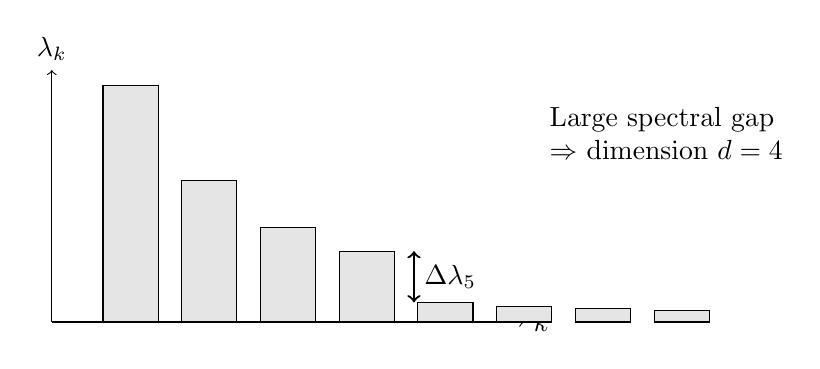
\begin{tikzpicture}[scale=1.0]
    \draw[->] (0,0) -- (6,0) node[right]{$k$};
    \draw[->] (0,0) -- (0,3.2) node[above]{$\lambda_k$};
    \foreach \k/\h in
      {1/3.0,2/1.8,3/1.2,4/0.9,5/0.25,6/0.20,
       7/0.17,8/0.15} {
      \draw[fill=black!10]
        (\k-0.35,0) rectangle (\k+0.35,\h);
    }
    \draw[<->, thick]
      (4.6,0.9) -- (4.6,0.25)
      node[midway,right]{$\Delta\lambda_5$};
    \node[align=left, anchor=west] at (6.2,2.4)
      {Large spectral gap\\
       $\Rightarrow$ dimension $d=4$};
  \end{tikzpicture}
  \caption{Schematic eigenvalue spectrum for intrinsic
    dimension selection.
    A clear gap after four modes indicates a robust $d=4$
    projectable regime.}
  \label{fig:eigenvalue-gap}
\end{figure}

Failure of the reconstruction (non-local connectivity or no clear
spectral gap) signals a transition to a pre-geometric regime where a
smooth manifold is not an adequate description.
The effective metric is defined implicitly through propagation properties
and carries only a restricted subset of the relational information.
Poisson-type and wave-like equations arise from linearizing relaxation
dynamics around quasi-homogeneous configurations; they are
regime-dependent approximations, not fundamental laws.
